

\subsection{Convergence analysis in 3D}

Inspired by the convergence test in 2D we test our code on the problem 

\begin{align}
f_x = &K^* \left[-2(y^2-1)(z^2-1) + (2 \nu -1)(x^2-1)(z^2 +y^2-2) \right.\nonumber\\
 &\left. -2x(y(z^2-1) + z(y^2-1)) \right] \\
 f_y = &K^* \left[-2(x^2-1)(z^2-1) + (2 \nu -1)(y^2-1)(z^2 +x^2-2) \right.\nonumber\\
 &\left. -2y(x(z^2-1) + z(x^2-1)) \right] \\
 f_z = &K^* \left[-2(x^2-1)(y^2-1) + (2 \nu -1)(z^2-1)(y^2 +x^2-2) \right.\nonumber\\
 &\left. -2z(x(y^2-1) + y(x^2-1)) \right] \\
 K^* = & \frac{E \nu}{(1+\nu)(1-2\nu)},
\end{align}
on the reference cube $(-1,1)^3$ with homogeneous Dirichlet boundary conditions on all boundaries. This problem has the analytical solution

\begin{align}
\bm{u} = \begin{bmatrix}
\, (x^2-1)(y^2-1)(z^2-1) \, \\
\, (x^2-1)(y^2-1)(z^2-1) \, \\
(x^2-1)(y^2-1)(z^2-1)
\end{bmatrix}.
\end{align}
As can be seen in Figure \ref{fig:convergence3d}, the convergence is linear.

\begin{figure}
\center
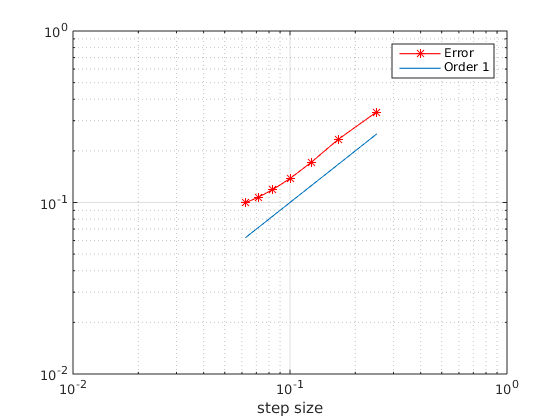
\includegraphics[width=0.4\textwidth]{convergence3d}
\caption{Logarithm error convergence plot for the 3d case, with N = 4, 6, 8, 10, 12, 14, 16 grid points in each spatial direction.}
\label{fig:convergence3d}
\end{figure}

